\documentclass[11pt]{article}

\usepackage{acl}
\usepackage{times}
\usepackage{latexsym}
\usepackage[T1]{fontenc}
\usepackage[utf8]{inputenc}
\usepackage{microtype}
\usepackage{graphicx}
\usepackage{booktabs}
\usepackage{amsmath}
\usepackage{array}
\usepackage{multirow}
\usepackage{xurl}
\usepackage{xcolor}


\newcommand{\cl}{\textsc{Confident Learning}}
\newcommand{\cleanlab}{\texttt{cleanlab}}

\title{Reproducing and Extending Confident Learning\\
for Detecting Label Errors in Classification Data}

\author{
  Md Maruf Khan \\
  Student ID: 48627070 \\
  Macquarie University
}

\begin{document}
\maketitle

\begin{abstract}
Confident learning (CL) estimates and ranks label errors using out-of-sample
class probabilities. This project first reproduces a released CIFAR-10
benchmark from Northcutt et al. and then tests how well the method
generalises beyond the paper's synthetic benchmark. Running the original
\cleanlab{} v0.1.0 on the authors' released probabilities regenerated all
five released label-error masks bit-for-bit in the main setting, reproducing the paper's
confident-joint result exactly (precision 0.771, recall 0.836, $F_1$ 0.802);
45 of 60 masks across all twelve noise/sparsity settings were identical and
the rest differed on at most 9 of 50,000 examples. The paper's
joint-estimation RMSE was also reproduced: all 24 values in its
Table~S1 were matched after rounding. Current \cleanlab{}
2.9.0 yields $F_1=0.790$ with 98.5\% mask agreement, a measurable
software-version effect in the filtering step. Extensions used real human annotations from CIFAR-10N and CIFAR-100N,
and a new controlled text dataset, AGNews-CLNoise. On the full 50,000-image
CIFAR-10N aggregate labels, CL achieved $F_1=0.546$; on a balanced 10,000-image
CIFAR-100N subset it achieved $F_1=0.650$. On AGNews-CLNoise, the original
20\% cyclic setting achieved $F_1=0.800$, while a 24-run sensitivity study
showed that performance depended strongly on the structure of corruption and
the classifier supplying predicted probabilities. A blind human review and a
pinned, order-reversed Qwen judge further showed that semantic review can
explain apparent false positives, but that an LLM judge is position-sensitive.
All scripts, derived data, source revisions, results, and deterministic hashes
are released in a public repository.
\end{abstract}

\section{Introduction and Paper Justification}

Supervised classifiers normally treat dataset labels as ground truth, even
though labels may be wrong because of annotation mistakes, ambiguous examples,
automatic collection, or overlapping class definitions. A label-error detector
therefore has two related goals: estimate how much noise exists and identify
which individual examples should be reviewed.

Northcutt et al. propose \cl{}, a model-agnostic framework that estimates the
joint distribution between observed noisy labels and latent true labels using
out-of-sample predicted probabilities \citep{northcutt2021confident}. CL uses
class-specific confidence thresholds to count confident disagreements,
constructs a \emph{confident joint}, and then ranks or prunes suspected label
issues. The paper makes three claims relevant to this project: (1) under stated
conditions CL consistently estimates the noisy--true label joint and can
exactly identify errors; (2) it is not tied to one classifier or modality; and
(3) removing suspected errors can improve learning with noisy labels. The
original evaluation combines controlled CIFAR-10 corruption with qualitative
and downstream studies on images and text.

The paper is a strong basis for a novel replication project on several
independent criteria. \emph{Venue quality:} it appeared in the refereed,
diamond-open-access \emph{Journal of Artificial Intelligence Research} (JAIR),
which the CORE2020 journal ranking (CORE's final journal list) rates
\textbf{A}.\footnote{Paper:
\url{https://www.jair.org/index.php/jair/article/view/12125}; CORE ranking:
\url{https://portal.core.edu.au/jnl-ranks/145/}.} \emph{Impact:} Google
Scholar listed 1,557 citations as of 8~November 2026, and the method
underlies the widely used open-source \cleanlab{} library.
\emph{Reproducibility:} the authors released code, the exact noisy labels,
out-of-sample probabilities, and every method's output mask, so each stage of
the result can be checked. \emph{Relevance:} its modality-independent claim
creates a meaningful extension question: does the procedure retain useful
error-detection performance under real human noise and under a new text
construction?

This report addresses four research questions:

\begin{enumerate}
  \item Can the released CIFAR-10 label-error results be reproduced from the
  authors' artifacts, and how does the current software behave on them?
  \item How does CL perform on real human annotations in CIFAR-10N and
  CIFAR-100N?
  \item How stable is CL on a controlled text dataset when noise rate, noise
  structure, random seed, and classifier are varied?
  \item Can blind human review and a reproducible LLM judge clarify disputed
  labels without being treated as infallible ground truth?
\end{enumerate}

\section{Original Work and Data}

\subsection{Method and evaluation framework}

Let $\tilde{y}$ denote the observed label and $y^*$ the unknown true label.
Given out-of-sample class probabilities $\hat{p}(y=j\mid x)$, CL calculates a
confidence threshold for each observed class and counts examples that
confidently support a different class. These counts are calibrated to estimate
$P(\tilde{y}=i,y^*=j)$. Entries away from the diagonal correspond to possible
label transitions. Crucially, cross-validation is used so that an example is
not judged by a model trained on that same example.

The original paper evaluates three questions. First, on synthetic CIFAR-10
noise, root mean squared error measures estimation of the known noisy--true
joint. Second, individual error detection is evaluated by precision, recall,
and $F_1$ \citep{sokolova2009systematic}:
\begin{equation}
\begin{aligned}
P&=\frac{TP}{TP+FP}, &
R&=\frac{TP}{TP+FN},\\
F_1&=\frac{2PR}{P+R}.
\end{aligned}
\end{equation}
Third, classifiers are retrained after suspected errors are removed and
evaluated by held-out accuracy. The original CIFAR-10 study varies label-noise
rate and transition-matrix sparsity and compares five CL variants with several
noisy-label baselines. The most computationally expensive downstream results
average ten ResNet-50 trials; those full training trials were outside the CPU
budget of this project.

On its own benchmark the method was highly successful. For joint estimation
at 20\% and 40\% noise, CL averaged an RMSE of 0.004 against the true joint,
versus 0.006 for the simpler confusion-matrix estimate. For label-error
detection on CIFAR-10, the authors' released confident-joint masks give $F_1$
between 0.69 and 0.84 across the twelve released noise/sparsity settings,
including $P=0.771$, $R=0.836$, $F_1=0.8025$ at 40\% noise and 60\% sparsity,
the values reported in the paper's Table~4. For downstream learning (the paper's Table~2), training on
CL-cleaned data at 40\% noise and 60\% sparsity reached 87.2\% CIFAR-10 test
accuracy for the best variants (PBNR and C+NR) and 86.9\% for the confident
joint, compared with 73.6\% for INCV, the strongest non-CL baseline, and
57.3\% for training on the noisy labels directly.

The extensions additionally report Matthews correlation coefficient (MCC),
which uses all four confusion-matrix cells and is useful when errors are rare
\citep{matthews1975comparison}, and average precision (AP), which evaluates the
ranking induced by $1-$label-quality score. ``Lift'' is reported only as
precision divided by error prevalence: it measures how concentrated true
errors are in the flagged set relative to random selection, not ranking
quality.

\subsection{Datasets in the original paper}

Table~\ref{tab:original-data} summarises every dataset used in the original
paper. CIFAR-10 is the main quantitative error-detection benchmark because its
synthetic corruption provides known ground truth. The other datasets test
different scales, modalities, or naturally occurring label problems.

\begin{table*}[t]
\centering
\small
\setlength{\tabcolsep}{4pt}
\renewcommand{\arraystretch}{1.08}
\begin{tabular}{p{2.35cm}p{2.6cm}p{4.0cm}p{5.9cm}}
\toprule
\textbf{Dataset} & \textbf{Scale / format} & \textbf{Role in the paper} & \textbf{Important preparation} \\
\midrule
CIFAR-10 \citep{krizhevsky2009learning}
& 60,000 $32\!\times\!32$ RGB images, 10 classes
& Joint estimation, error detection, and downstream learning
& The 50,000 training labels are corrupted with asymmetric class-conditional matrices; the 10,000 test labels remain unchanged. \\
ImageNet \citep{russakovsky2015imagenet}
& 1.28M training and 50,000 validation images, 1,000 classes
& Real label/ontology problems and filtered retraining
& ResNet-18/50 predictions are used; targeted cleaning is compared with random removal. \\
MNIST \citep{lecun1998gradient}
& 70,000 greyscale digit images, 10 classes
& Errors in a dataset often assumed clean
& A small CNN produces cross-validated probabilities; examples are ranked by self-confidence. \\
WebVision \citep{li2017webvision}
& More than 1M web images, 1,000 classes
& Large-scale qualitative error discovery
& A pretrained ResNeXt supplies probabilities; CL ranks likely errors without retraining on WebVision. \\
Amazon Reviews \citep{he2016ups}
& Approximately 10M filtered reviews, 3 sentiment classes
& Text, class imbalance, and non-deep classification
& Two- and four-star reviews are removed; five-fold multinomial logistic regression uses fastText representations. \\
\bottomrule
\end{tabular}
\caption{Original datasets and their distinct evaluation roles.}
\label{tab:original-data}
\end{table*}

CIFAR-10 itself is distributed as binary batches of 32$\times$32 colour images
with integer class labels; the authors' artifact stores the training images as
PNG files in one folder per class.\footnote{CIFAR-10:
\url{https://www.cs.toronto.edu/~kriz/cifar.html}.} The authors' released
replication artifact\footnote{Authors' artifact repository (commit
\texttt{2f31556}):
\url{https://github.com/cgnorthcutt/confidentlearning-reproduce}.} wraps it
in a linked set of files for each of the twelve noise/sparsity settings: (i)
a JSON mapping from each training-image path to its noisy class, where the
path's folder name encodes the clean class; (ii) a $50{,}000\times10$ float16
matrix of four-fold out-of-sample ResNet-50 probabilities; and (iii) for each
of five methods, a 50,000-element Boolean keep mask. Table~\ref{tab:orig-snippet}
shows genuine rows from the 40\%-noise, 60\%-sparsity setting, one for each
outcome type.

\begin{table}[t]
\centering
\small
\setlength{\tabcolsep}{2.4pt}
\begin{tabular}{rllrrrc}
\toprule
\textbf{Row} & \textbf{Clean} & \textbf{Noisy} & \textbf{$\hat{p}_{\text{noisy}}$} & \textbf{$\hat{p}_{\text{clean}}$} & \textbf{$\max\hat{p}$} & \textbf{Kept?} \\
\midrule
1 & airplane & automobile & .068 & .642 & .642 & no (TP) \\
0 & airplane & airplane & .208 & .208 & .473 & no (FP) \\
30 & airplane & automobile & .205 & .131 & .458 & yes (FN) \\
18 & airplane & airplane & .355 & .355 & .355 & yes (TN) \\
\bottomrule
\end{tabular}
\caption{Genuine rows of the released CIFAR-10 artifact (40\% noise, 60\%
sparsity). ``Row'' is the array index; e.g.\ row~1 is image
\texttt{airplane/10010\_airplane.png} with JSON noisy label~1 (automobile).
$\hat{p}$ values are ResNet-50 probabilities; ``Kept?'' is the confident-joint
keep mask, with the outcome relative to the clean label.}
\label{tab:orig-snippet}
\end{table}

\section{Replication of the Original Work}
\label{sec:replication}

\subsection{Scope and environment}

The replication has three stages, all on the authors' released data at
artifact commit \texttt{2f31556}; scripts, outputs, and hashes are in the
public project repository.\footnote{
\url{https://github.com/marufkhan09/comp8240-confident-learning}. All
results and scripts in this report correspond to repository commit
\texttt{8577ccc}.}

\emph{Stage 1 (evaluate released outputs).} For the 40\%-noise, 60\%-sparsity
setting (50,000 images; 19,981 actual corruptions, 39.96\%), the script
reconstructs clean labels from image paths, inverts each released keep mask
to a flagged-error mask, and recomputes TP, FP, FN, $P$, $R$, and $F_1$.

\emph{Stage 2 (run the original code).} The artifact README states that the
paper used \cleanlab{} v0.1.0. That version predates current NumPy, so it was
run in an isolated Python 3.11.18 environment (NumPy 1.23.5, scikit-learn
1.2.2, SciPy 1.10.1). The script makes exactly the calls in the authors' work
log (\texttt{compute\_confident\_joint} and \texttt{get\_noise\_indices} with
each pruning method) on the unmodified float16 probabilities, for all twelve
released settings, and compares every regenerated mask with the released one.

\emph{Stage 3 (current software).} The five methods were re-run with
\cleanlab{} 2.9.0 (Python 3.12.1, NumPy 2.5.2, scikit-learn 1.9.0, GitHub
Codespace). Because the float16 rows sum to 0.9868--1.0000 and the current
library validates its inputs, they were converted to float64 and
renormalised for this stage only.

\emph{Stage 4 (joint estimation).} Following the authors' work log, the
true joint is the released noise matrix multiplied by the clean-label prior,
$Q_{\tilde{y},y^*}=P(\tilde{y}\mid y^*)\,P(y^*)$; $\hat{Q}$ is obtained from
\texttt{estimate\_joint} using either the confident joint or the
argmax confusion matrix ($C_{\text{confusion}}$), and
$\text{RMSE}=\big(\frac{1}{m^2}\sum_{i,j}(\hat{Q}_{ij}-Q_{ij})^2\big)^{1/2}$.
This was run in both environments for all twelve settings.

The scope is deliberately the joint-estimation and label-error detection
results, not the paper's ten-trial ResNet-50 retraining benchmark, which
exceeds the CPU budget.
Reusing the released out-of-sample probabilities isolates CL's counting and
filtering behaviour, which is the paper's methodological contribution.

\subsection{Replication results}

\begin{table}[t]
\centering
\small
\setlength{\tabcolsep}{3.8pt}
\setlength{\tabcolsep}{3pt}
\begin{tabular}{lrrrrr}
\toprule
\textbf{Method} & \textbf{Paper} & \textbf{Released} & \textbf{v0.1.0} & \textbf{v2.9.0} & \textbf{Agree} \\
\midrule
$C_{\text{confusion}}$ & .79 & .7880 & .7880 & .7879 & 99.98\% \\
$C_{\tilde{y},y^*}$ & .80 & \textbf{.8025} & \textbf{.8025} & .7900 & 98.51\% \\
PBC & .79 & .7946 & .7946 & .7945 & 99.96\% \\
PBNR & .80 & .8004 & .8004 & .8002 & 99.97\% \\
C+NR & .78 & .7830 & .7830 & .7829 & 99.95\% \\
\bottomrule
\end{tabular}
\caption{$F_1$ at 40\% noise, 60\% sparsity: the paper's Table~4 (two
decimals, as printed), the authors' released masks, masks regenerated with
the original \cleanlab{} v0.1.0 (all five identical to the released masks),
and current \cleanlab{} 2.9.0 with its example-wise agreement with the
released mask. $C_{\text{confusion}}$ is the argmax-disagreement method;
$C_{\tilde{y},y^*}$ is the confident joint; C+NR is ``both''.}
\label{tab:replication}
\end{table}

\begin{table*}[t]
\centering
\small
\setlength{\tabcolsep}{5pt}
\begin{tabular}{lcccc}
\toprule
 & \textbf{20\% / 0.0} & \textbf{20\% / 0.6} & \textbf{40\% / 0.0} & \textbf{40\% / 0.6} \\
\textbf{Method} & paper\,|\,ours & paper\,|\,ours & paper\,|\,ours & paper\,|\,ours \\
\midrule
$C_{\text{confusion}}$ & 71\,|\,70.9 & 72\,|\,72.4 & 84\,|\,84.0 & 79\,|\,78.8 \\
$C_{\tilde{y},y^*}$ & 75\,|\,75.0 & 78\,|\,77.7 & 84\,|\,83.6 & 80\,|\,80.2 \\
PBC & 76\,|\,76.4 & 76\,|\,76.1 & 84\,|\,84.4 & 79\,|\,79.5 \\
PBNR & 77\,|\,76.7 & 79\,|\,78.7 & 85\,|\,85.0 & 80\,|\,80.0 \\
C+NR & 78\,|\,78.1 & 78\,|\,78.1 & 84\,|\,84.2 & 78\,|\,78.3 \\
\bottomrule
\end{tabular}
\caption{Every setting in the paper's Table~4 (noise / sparsity): reported
$F_1$ (\%, as printed) versus $F_1$ of the released masks,
which \cleanlab{} v0.1.0 regenerates. All 20 $F_1$ values agree after
rounding. Across all 60 reported precision, recall, and $F_1$ values, 59 round
to the printed value. The sole exception is PBC precision at 20\% noise and
0.0 sparsity: 0.6349 from the released artifact versus 0.64 in the paper, a
difference of 0.0051.}
\label{tab:paper-table4}
\end{table*}

\begin{table}[t]
\centering
\small
\setlength{\tabcolsep}{5pt}
\begin{tabular}{lrrrr}
\toprule
\textbf{Noise} & \multicolumn{4}{c}{\textbf{Sparsity}} \\
\cmidrule(l){2-5}
 & \textbf{0.0} & \textbf{0.2} & \textbf{0.4} & \textbf{0.6} \\
\midrule
20\% & .750 & .753 & .787 & .777 \\
40\% & .836 & .828 & .842 & .803 \\
70\% & .828 & .836 & .782 & .689 \\
\bottomrule
\end{tabular}
\caption{Confident-joint $F_1$ in all twelve released settings. Masks
regenerated with \cleanlab{} v0.1.0 were identical to the released masks in
every setting.}
\label{tab:replication-grid}
\end{table}

\paragraph{Results and closeness.} For the released confident-joint mask,
$TP=16{,}710$, $FP=4{,}955$, and $FN=3{,}271$, giving $P=0.7713$,
$R=0.8363$, and $F_1=0.8025$, matching the paper's Table~4 (77\%, 84\%,
80\%). The paper's Table~4 reports four settings; Table~\ref{tab:paper-table4}
compares all of them, and every reported $F_1$ is matched after rounding.
The comparison is restricted to these four noise--sparsity combinations; the
remaining eight released configurations (Table~\ref{tab:replication-grid})
are reported separately and are not presented as replications of a paper
table. Running the
original code reproduced the method itself, not only its outputs: with
\cleanlab{} v0.1.0, all five masks in the main setting were bit-for-bit
identical to the released masks (Table~\ref{tab:replication}). Across all
twelve settings, 45 of the 60 regenerated masks were identical, including the
confident-joint mask in every setting (Table~\ref{tab:replication-grid}). The
other 15 (seven CL-PBNR, seven CL-both, and one argmax mask)
differed from the released mask on at most 9 of 50,000 examples, changing
$F_1$ by at most 0.0002. These residual differences were deterministic across
our runs, so they are most plausibly tie-breaking effects of the original
computing environment rather than a methodological discrepancy; they were not
investigated further.

\paragraph{Why current software differs.} Under \cleanlab{} 2.9.0, four
methods are essentially unchanged, but the confident-joint mask differs from
the released mask on 746 examples (98.51\% agreement) and its $F_1$ falls to
0.7900. The two runs did not receive literally identical inputs, because only
the modern path required float64 renormalisation. This was tested directly:
running \cleanlab{} v0.1.0 on the same renormalised probabilities changes
only 18 of 50,000 mask decisions and reduces $F_1$ only from 0.8025 to
0.8024. Renormalisation therefore explains a negligible part of the
discrepancy: even if every one of those 18 changes overlapped with
\cleanlab{} 2.9.0's, at least 728 of its 746 differences remain. Most of the
gap is associated with changes in the modern \cleanlab{} implementation and
its software environment, not with the data, the released masks, the metric
calculation, or an error in the paper. Reporting all three columns separates repeatability of the artifact,
reproducibility of the method, and robustness to software change.

\begin{table}[t]
\centering
\small
\setlength{\tabcolsep}{4pt}
\begin{tabular}{llrrrr}
\toprule
 & & \multicolumn{4}{c}{\textbf{Sparsity}} \\
\cmidrule(l){3-6}
\textbf{Noise} & \textbf{Count} & \textbf{0.0} & \textbf{0.2} & \textbf{0.4} & \textbf{0.6} \\
\midrule
\multirow{2}{*}{20\%} & $C_{\tilde{y},y^*}$ & .0042 & .0041 & .0036 & .0037 \\
 & $C_{\text{confusion}}$ & .0058 & .0056 & .0049 & .0055 \\
\multirow{2}{*}{40\%} & $C_{\tilde{y},y^*}$ & .0040 & .0043 & .0041 & .0052 \\
 & $C_{\text{confusion}}$ & .0049 & .0051 & .0055 & .0070 \\
\multirow{2}{*}{70\%} & $C_{\tilde{y},y^*}$ & .0108 & .0102 & .0146 & .0174 \\
 & $C_{\text{confusion}}$ & .0112 & .0111 & .0151 & .0192 \\
\bottomrule
\end{tabular}
\caption{RMSE of the estimated joint $\hat{Q}$ (\cleanlab{} v0.1.0, released
probabilities). All 24 values round to the paper's Appendix Table~S1;
\cleanlab{} 2.9.0 agrees to within $10^{-5}$.}
\label{tab:rmse}
\end{table}

\paragraph{Joint estimation.} Table~\ref{tab:rmse} reproduces the paper's
first evaluation question. All 24 RMSE values match the paper's Table~S1
after rounding to three decimals. Averaged over the eight 20\% and 40\%
settings, the confident joint gives 0.0042 and $C_{\text{confusion}}$ gives
0.0055, matching the paper's summary values of 0.004 and 0.006. The advantage
of the confident joint narrows at 70\% noise, as in the paper. Unlike the
error masks, the estimated joint is essentially unchanged under \cleanlab{}
2.9.0 (maximum difference $9\times10^{-6}$). This suggests that the 746-example
mask discrepancy above arises in the modern filtering step rather than in
counting or calibrating the confident joint.

All four stages produced identical outputs when re-run. The repository
README's Quickstart lists the command, downloads, and approximate CPU time for
every experiment in this report, and each script saves its output hashes.

\section{Construction of New Data}
\label{sec:new-data}

The extension was designed around two complementary forms of evidence. CIFAR-N
provides \emph{existing} real human annotation noise; AGNews-CLNoise is a
\emph{newly constructed} text benchmark with exactly known injected errors.
In every experiment, the model produces out-of-sample probabilities, CL flags
issues, and the flag is compared with a reference error mask.
Table~\ref{tab:pipeline} summarises the construction pipeline step by step;
the subsections explain the choices.

\begin{table*}[t]
\centering
\small
\setlength{\tabcolsep}{4pt}
\begin{tabular}{>{\raggedright\arraybackslash}p{2.3cm}>{\raggedright\arraybackslash}p{4.15cm}>{\raggedright\arraybackslash}p{4.15cm}>{\raggedright\arraybackslash}p{4.15cm}}
\toprule
\textbf{Step} & \textbf{CIFAR-10N} & \textbf{CIFAR-100N} & \textbf{AGNews-CLNoise} \\
\midrule
1. Source &
CIFAR-10 train images + CIFAR-N human labels (repo commit \texttt{49df7d8}) &
CIFAR-100 train images + CIFAR-N labels (same commit) &
AG News train split, 120,000 articles (HF revision \texttt{eb185aad}) \\
2. Alignment check &
CIFAR-N \texttt{clean\_label} must equal torchvision targets in order &
Same check against CIFAR-100 fine labels &
Text hashed (SHA-256); manifest stores index, labels, hash \\
3. Sampling &
Pilot: 5,000 images, stratified on aggregate labels, seed 42; full run: all 50,000 &
10,000 images, stratified on clean labels (100 per class), seed 42 &
10,000 articles, stratified (2,500 per class), seed 42 \\
4. Noisy labels &
Real: aggregate, worst-case, and three individual annotator label sets &
Real: official \texttt{noisy\_label} (coarse labels excluded) &
Injected: exactly $r\times2{,}500$ per class at $r\in\{10,20,30,40\}\%$, cyclic or symmetric, seeds 42--44 \\
5. Representation &
Resize to 96$\times$96, ImageNet normalisation, frozen ResNet-18 $\rightarrow$ 512-d features (cached) &
Same as CIFAR-10N &
TF--IDF, unigrams + bigrams, 30,000 features, sublinear TF \\
6. Probabilities &
Standardised logistic regression, stratified 4-fold out-of-sample, seed 42 &
Same as CIFAR-10N &
Logistic regression, the same 4 stratified folds for every run \\
7. Reference errors &
Noisy label $\neq$ CIFAR-N clean label &
Noisy label $\neq$ clean label &
Exactly the injected positions \\
\bottomrule
\end{tabular}
\caption{Construction pipeline for the new datasets. Each row is one processing
step; every random choice is seeded and recorded in the repository.}
\label{tab:pipeline}
\end{table*}

\subsection{CIFAR-10N and CIFAR-100N}

CIFAR-N adds Mechanical Turk labels to the original CIFAR training images
\citep{wei2022learning}. The official annotation repository was pinned at
commit \texttt{49df7d8}.\footnote{CIFAR-N labels:
\url{https://github.com/UCSC-REAL/cifar-10-100n}.} The image ordering was verified by checking that its
\texttt{clean\_label} array exactly matched the official torchvision targets.
This is important: a silent order mismatch would make every subsequent metric
meaningless.

For the CIFAR-10N pilot, a deterministic stratified subset of 5,000 images was
selected with seed 42. Images were resized to $96\times96$, normalised with
ImageNet statistics, and passed through a frozen ImageNet-pretrained ResNet-18.
The resulting 512-dimensional features were cached. A standardised logistic
regression model then generated four-fold out-of-sample probabilities. The
same cached images and the fold assignment derived from aggregate labels were
reused for all five human-label sets: aggregate, worst-case, and three
individual annotators. The full aggregate-label experiment used all 50,000
images and the same representation; caching the features makes repeat runs
fast on CPU.

For CIFAR-100N, a 10,000-image subset selected exactly 100 images from each of
100 fine-grained classes. The official \texttt{noisy\_label} was compared with
\texttt{clean\_label}; coarse labels were excluded because they define a
different 20-class task. The same frozen ResNet-18 and logistic-regression
pipeline was used, making the CIFAR-10N/CIFAR-100N comparison controlled with
respect to feature extraction and classifier family.

\subsection{AGNews-CLNoise}

AGNews-CLNoise was derived from the 120,000-example AG News training split
\citep{zhang2015character}, pinned to Hugging Face revision
\texttt{eb185aad}; the complete revision is recorded in the
repository.\footnote{AG News:
\url{https://huggingface.co/datasets/fancyzhx/ag_news}.} A
stratified sample of 10,000 articles contains 2,500 examples from each of
World, Sports, Business, and Sci/Tech. The source label is treated as the clean
reference, with the limitation that the original dataset may itself contain
ambiguity.

The baseline changes exactly 500 labels per class (2,000 total, or 20\%) using
the fixed cycle World$\rightarrow$Sports$\rightarrow$Business$\rightarrow$
Sci/Tech$\rightarrow$World. The follow-up sensitivity study keeps the same
articles and four folds while varying four noise rates (10--40\%), cyclic
versus symmetric corruption, and seeds 42--44. This produces 24 controlled
runs. Symmetric corruption randomly distributes each selected error over the
other three classes; cyclic corruption concentrates it in one competing class.
Each run generates four-fold probabilities with a TF--IDF (unigrams and
bigrams, 30,000-feature maximum) logistic-regression pipeline. An argmax
disagreement rule is included as a simple baseline.

Because the AG News dataset card listed its licence as unknown during the
project, raw text was downloaded only into the ignored \texttt{data/raw}
directory. The public manifest stores source indices, labels, and SHA-256 text
hashes, allowing integrity checks without republishing the articles. The
examples in Table~\ref{tab:data-snippet} illustrate the committed formats.

\begin{table*}[t]
\centering
\small
\setlength{\tabcolsep}{4pt}
\begin{tabular}{llrrrrlp{3.8cm}}
\toprule
\textbf{Source} & \textbf{Index} & \textbf{Clean} & \textbf{Noisy} & \textbf{Pred.} & \textbf{Flag} & \textbf{Score} & \textbf{Other stored metadata} \\
\midrule
CIFAR-10N & 19 & 6 & 6 & 0 & yes & .0005 & actual-error Boolean; original image index \\
CIFAR-100N & 1 & 29 & 63 & 29 & yes & $1.9{\times}10^{-8}$ & actual-error Boolean; original image index \\
AGNews & 14 & Business & Sci/Tech & Business & yes & .1561 & source index; text hash; run/seed \\
AGNews & 38 & Business & Sci/Tech & Sci/Tech & no & .8459 & source index; text hash; run/seed \\
\bottomrule
\end{tabular}
\caption{Snippets of the row-oriented derived data. ``Score'' is label
quality; lower values indicate more likely errors. Text and images remain in
their source datasets rather than being republished.}
\label{tab:data-snippet}
\end{table*}

\subsection{Blind annotation and LLM-judge protocol}

Thirty cases were sampled from CL flags that were \emph{not} deliberately
corrupted in the verified 20\%-cyclic AG News run---apparent false positives
under the synthetic reference. Sampling was approximately balanced across the
four source classes. In a blind review, the human annotator saw the article and
two randomly ordered candidates: the original AG News label and the model's
alternative. Their roles and earlier model decisions were hidden. The choices
were candidate A, candidate B, ambiguous, or neither. A three-category mapping
(original, alternative, ambiguous/neither) and agreement statistics were
written before the review. This is narrower than the proposal's plan of
about 100 cases stratified across TP, FP, FN, and TN. With a single annotator,
the review effort was concentrated on apparent false positives, the only
outcome whose correctness the synthetic reference cannot settle; true
positives and false negatives are decided by construction.

Because only one human annotator was available, an independently executed,
pinned, order-controlled LLM judge was used as a supplementary annotator. This
follows the unit's permitted LLM-as-judge approach but does not replace a
human--human reliability study. The judge was Qwen2.5-0.5B-Instruct
\citep{qwen2024qwen25}, pinned to revision \texttt{7ae5576}\footnote{Model:
\url{https://huggingface.co/Qwen/Qwen2.5-0.5B-Instruct}.} and run locally.
It replaced the proposal's tentative Prometheus~2 \citep{kim2024prometheus},
whose 7B+ models were impractical on the available CPU-only Codespace; local
execution also kept article text away from commercial APIs. The small judge
was a deliberate CPU-compatible trade-off and may have contributed to the
position sensitivity reported below; this cannot be isolated without
comparison to a larger judge. Each case was judged twice: pass~1 used a
deterministically random candidate order and pass~2 reversed it. The prompt
defined the four topics, hid label provenance, required A/B/AMBIGUOUS/NEITHER,
and requested one-sentence justification. Greedy decoding, the exact prompt,
model revision, seeds, and software versions were recorded. Raw text and raw
responses stayed private; the public output contains identifiers, hashes,
candidate roles, parsed choices, and consistency indicators. Cohen's $\kappa$
measures agreement beyond chance \citep{cohen1960coefficient}.

\section{Results on New Data}
\label{sec:results}

\subsection{Relation to the replication}

The replicated benchmark and the extensions differ in three deliberate ways,
so their numbers are related but not identical quantities. (1) \emph{Noise
source:} the replication's errors are synthetic class-conditional
corruptions with exact ground truth; CIFAR-N errors are real human
disagreements with a reference label that may itself be imperfect; AGNews
errors are synthetic again but in text. (2) \emph{Probability model:} the
replication uses the authors' four-fold ResNet-50 trained on the noisy
labels; the image extensions use a frozen ImageNet ResNet-18 with four-fold
logistic regression, and AGNews uses TF--IDF with four-fold logistic
regression. (3) \emph{Metrics:} the replication reports the paper's $P$,
$R$, and $F_1$; the extensions add MCC and AP because error prevalence
varies from 9\% to 40\% across datasets. Holding the CL step fixed while
changing the noise and the model is what allows the comparison in
Table~\ref{tab:main-results} to test the paper's generality claim.

At a matched 20\% noise rate, the replicated CIFAR-10 confident-joint $F_1$
ranges from 0.750 to 0.787 across sparsities (Table~\ref{tab:replication-grid}),
and the constructed AGNews benchmark with 20\% cyclic noise gives a comparable
$F_1=0.800$. This supports the claim that CL transfers across modalities when
the noise is synthetic and the classifier is adequate. At 40\% the picture
splits: CIFAR-10 stays at 0.803--0.842, AGNews symmetric noise is similar
(0.847), but AGNews cyclic noise falls to 0.664 (Section~\ref{sec:sweep}).
Real human noise is harder: CIFAR-10N and CIFAR-100N reach $F_1$
of 0.546 and 0.650, mainly through lower precision.

\subsection{Real human annotation noise}

\begin{table*}[t]
\centering
\small
\setlength{\tabcolsep}{4pt}
\begin{tabular}{lrrrrrrrrr}
\toprule
\textbf{Dataset / scope} & \textbf{$n$} & \textbf{Errors} & \textbf{Flags} & \textbf{$P$} & \textbf{$R$} & \textbf{$F_1$} & \textbf{MCC} & \textbf{AP} & \textbf{Clean acc.} \\
\midrule
\emph{Replication: CIFAR-10 synthetic} & 50,000 & 19,981 & 21,665 & .771 & .836 & .802 & --- & --- & --- \\
\midrule
CIFAR-10N aggregate pilot & 5,000 & 466 & 1,431 & .248 & .762 & .374 & .337 & .427 & .692 \\
CIFAR-10N aggregate full & 50,000 & 4,505 & 5,878 & .482 & .629 & .546 & .499 & .647 & .820 \\
CIFAR-100N fine pilot & 10,000 & 3,954 & 6,329 & .528 & .845 & .650 & .356 & .692 & .364 \\
AGNews 20\% cyclic & 10,000 & 2,000 & 2,251 & .756 & .851 & .800 & .749 & .730 & .856 \\
\bottomrule
\end{tabular}
\caption{Main extension results, with the replicated confident-joint result
(40\% noise, 60\% sparsity) as the reference row. For CIFAR-N, ``errors'' are
disagreements between human noisy labels and released clean references; for
CIFAR-10 and AGNews they are injected corruptions. MCC, AP, and accuracy are
not available for the released masks, which store no scores.}
\label{tab:main-results}
\end{table*}

Table~\ref{tab:main-results} shows that the strong synthetic result does not
transfer unchanged to real human annotations. In the 5,000-image CIFAR-10N
pilot, CL recovered 355 of 466 disagreements but also flagged 1,076 cases that
matched the clean reference, producing high recall (0.762) and low precision
(0.248). On all 50,000 aggregate labels, precision and $F_1$ rose to 0.482 and
0.546 while recall fell to 0.629. Because this is one fixed pilot subset rather
than a randomised sample-size experiment, the difference is an association,
not a causal estimate of the benefit of more data.

Across the five CIFAR-10N label sets, $F_1$ ranged from 0.374 (aggregate,
9.3\% disagreement prevalence) to 0.664 (worst-case, 40.5\% prevalence), while
MCC stayed in the narrower 0.337--0.390 range. Thus, the higher $F_1$ for the
worst-case labels partly reflects that a flagged example is more likely to be
wrong when errors are common; it does not by itself show easier intrinsic
detection. CIFAR-100N had high recall (0.845) but modest MCC (0.356), suggesting
that CL found most disagreements at the cost of many flags. The much lower
clean-label classification accuracy (0.364) also makes this 100-class task
harder for the frozen-feature classifier.

\subsection{Controlled text sensitivity study}
\label{sec:sweep}

The 20\%-cyclic AG News baseline recovered 1,701 of 2,000 injected errors and
exactly reproduced the original pilot counts. Across all 24 runs, CL had higher
mean $F_1$ than argmax disagreement in seven of eight aggregate configurations
(Figure~\ref{fig:agnews-sweep}), although at 40\% noise both differences
are within seed-to-seed variation (cyclic 0.6636 versus 0.6611; symmetric
0.8468 versus 0.8480). The largest advantage occurs at 10\% noise, where
errors are rare.

\begin{figure*}[t]
\centering
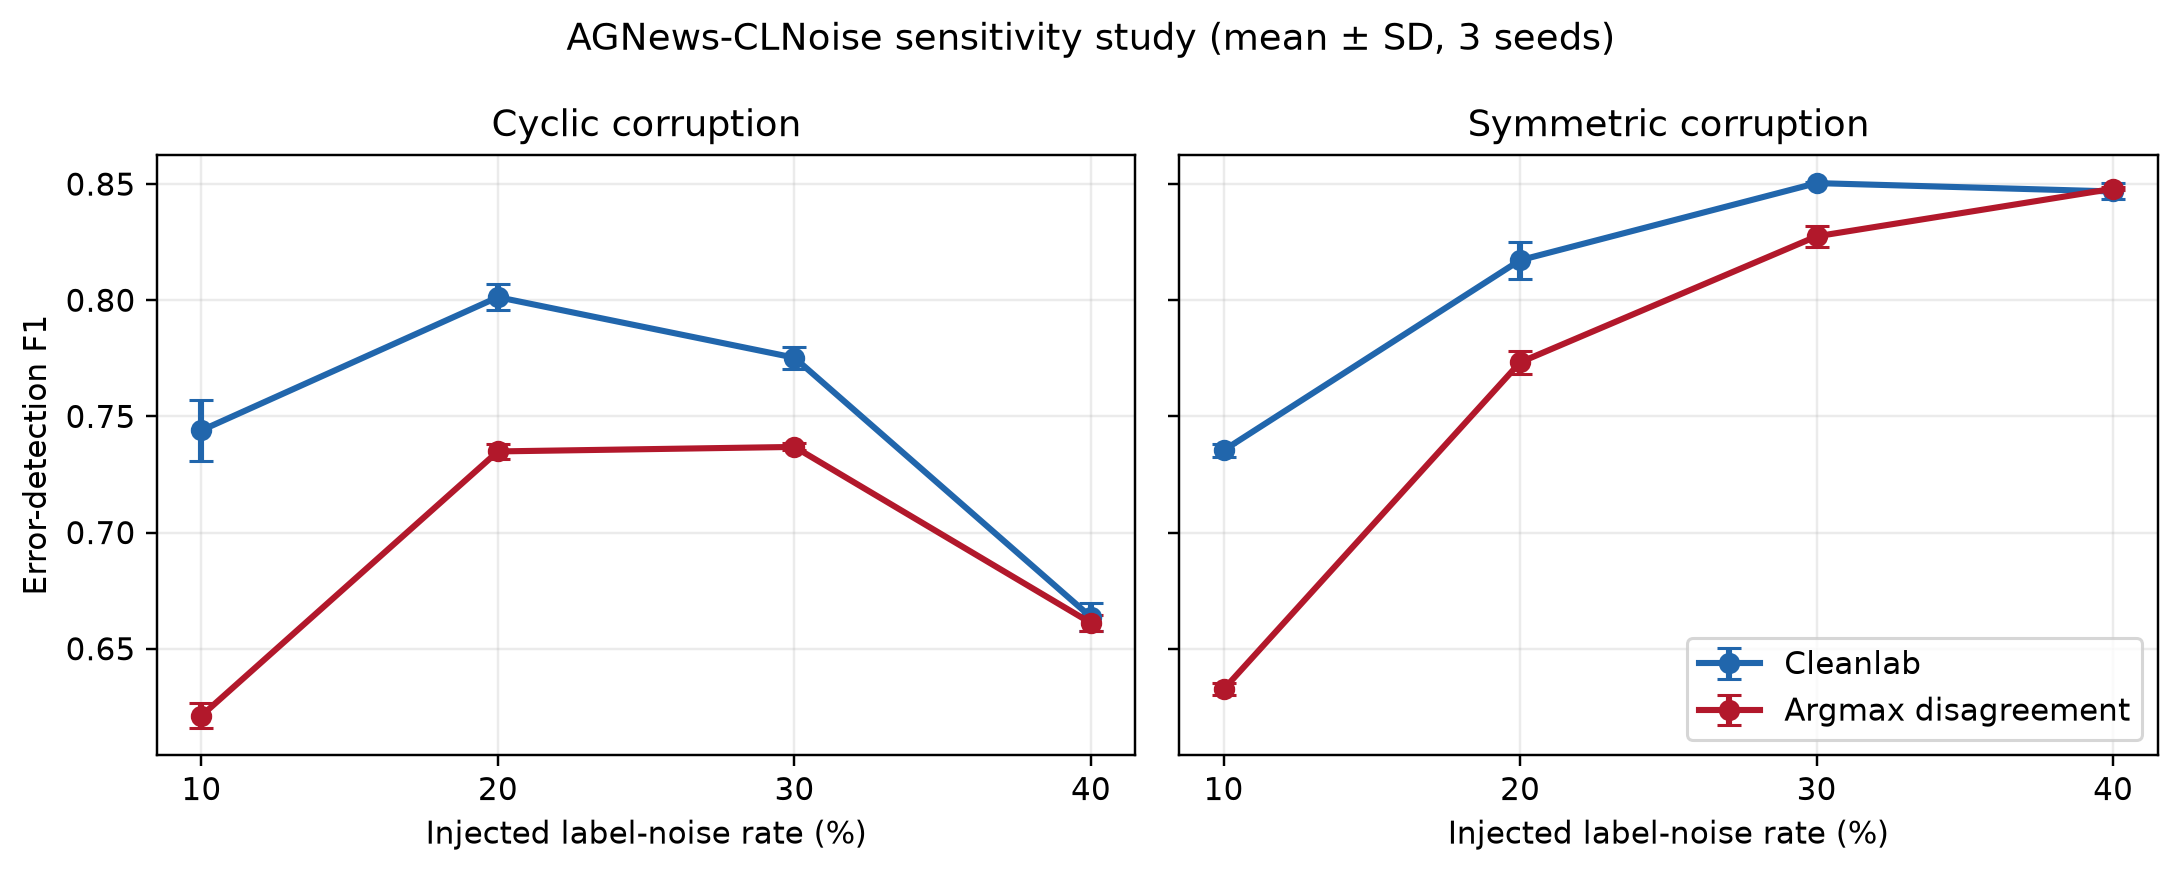
\includegraphics[width=0.96\textwidth]{figures/agnews_noise_sweep_f1.png}
\caption{AGNews-CLNoise sensitivity study. Points are means and error bars are
standard deviations over corruption seeds 42--44. Articles and folds are held
fixed.}
\label{fig:agnews-sweep}
\end{figure*}

The most informative failure is 40\% cyclic corruption: CL's mean $F_1$ falls
to 0.6636, compared with 0.8468 under symmetric noise. A plausible explanation
is that cyclic noise concentrates all changed labels from one class into the
same alternative, creating a strong competing mapping that the classifier can
learn; symmetric noise spreads those changes across three alternatives. This
is an interpretation of the controlled observation, not a general causal
claim about all text datasets. It also shows why reporting only one synthetic
noise mechanism would overstate generality.

Classifier choice mattered even when articles, folds, rates, structures, and
seeds were fixed. At 20\% cyclic/symmetric noise, mean CL $F_1$ was
0.801/0.817 for logistic regression, 0.838/0.834 for Complement Naive Bayes,
and 0.777/0.802 for calibrated linear SVM. Complement Naive Bayes was best in
this experiment, but the broader conclusion is more cautious: CL is
model-agnostic as an algorithm, yet its empirical quality depends on the
probabilities supplied by the underlying classifier.

\subsection{Human annotation and LLM-as-judge}

The blind human reviewer selected the original label in 15 cases and the
model-supported alternative in 15; no case was assigned ambiguous/neither.
This result indicates that some apparent false positives under the synthetic
reference may be genuine semantic problems in the original AG News labels.
However, one annotator and 30 deliberately disputed cases cannot estimate the
dataset-wide error rate.

\begin{table}[t]
\centering
\small
\setlength{\tabcolsep}{4pt}
\begin{tabular}{lrrr}
\toprule
\textbf{Qwen comparison} & \textbf{$n$} & \textbf{Agree} & \textbf{$\kappa$} \\
\midrule
Pass 1 vs human & 30 & 76.7\% & .533 \\
Pass 2 vs human & 30 & 63.3\% & .313 \\
Consistent subset vs human & 14 & 92.9\% & .837 \\
\bottomrule
\end{tabular}
\caption{Formal Qwen judge agreement with the blind human review. The
consistent subset is selected and is not an overall accuracy estimate.}
\label{tab:qwen}
\end{table}

All 60 formal Qwen responses were parseable, but only 14 of 30 cases (46.7\%)
received the same semantic decision after candidate order was reversed.
Table~\ref{tab:qwen} therefore gives two distinct messages. First, agreement
with the human judgement is positive and, on the order-consistent subset,
strong. Second, the large pass difference and low order consistency reveal
position sensitivity. The 92.9\% consensus agreement is calculated only after
selecting stable cases and must not be presented as judge accuracy on all 30.
The judge is useful for prioritising or explaining cases, but the results do
not support replacing independent human inspection.

As an additional external check, the released Mechanical Turk records from a
follow-up CL study \citep{northcutt2021labelerrors} were re-aggregated for seven
single-label test sets. All published counts were reproduced exactly: 4,835
human-validated errors among 11,813 CL-flagged candidates. These percentages
are conditional on prior CL selection and are not overall dataset error rates.
The analysis is supplementary because it reproduces a follow-up paper rather
than the central 2021 JAIR experiment.

\section{Ethical Considerations}

The Australian Code for the Responsible Conduct of Research emphasises
honesty, rigour, transparency, fairness, respect, and accountability
\citep{australiancode2018}. These principles affect both the original work and
this extension.

\paragraph{Issues in the original paper.}
The paper's main benchmark inherits the provenance of its data. CIFAR-10 was
drawn from the 80 Million Tiny Images collection \citep{torralba2008tiny},
which its creators withdrew in 2020 after an audit found derogatory class
labels and offensive images \citep{prabhu2021pyrrhic}; CIFAR-10's ten classes
are benign, but its images were collected from web search without consent.
ImageNet, used for the paper's real-noise study, has documented problems in
its person categories that required later filtering \citep{yang2020fairer}.
WebVision is scraped from the web and Amazon Reviews consists of
user-generated text, raising copyright and consent questions about reusing
content for purposes its authors never anticipated. The paper also frames
removal of suspected errors as beneficial; if applied to data about people,
automatic pruning could silently delete legitimate but atypical examples and
shift error rates onto under-represented groups. On the positive side, the
paper is open access and releases code and intermediate artifacts, which is
what made this independent check possible and reflects the Code's emphasis
on transparency and open dissemination.

\paragraph{Labels are claims, not facts.}
Calling an example a ``label error'' can conceal legitimate ambiguity,
multi-label content, or a weak ontology. Automatic deletion could
disproportionately remove unusual or minority examples that a classifier finds
difficult. The original paper partly recognises ontology overlap, but any
deployment should treat CL flags as review priorities rather than automatic
proof. This report therefore uses ``disagreement'' for CIFAR-N and preserves an
ambiguous/neither option in semantic review.

\paragraph{Human and LLM annotation.}
The blind annotation sample is small and has one human reviewer, so it cannot
serve as definitive ground truth. The LLM judge may reproduce training-data
bias, misunderstand short articles, and prefer the first or second option.
Order reversal exposed this last risk directly. Reporting both passes,
invalid-output checks, $\kappa$, and selection of the consensus subset is more
honest than reporting only the most favourable agreement number. Human review
should remain the final decision point for consequential relabelling.

\paragraph{Provenance, licensing, and privacy.}
Source datasets and commits are recorded, but availability does not imply
permission to redistribute every item. Because the AG News licence was unclear,
raw articles were not committed; public files contain source indices and text
hashes. Likewise, CIFAR images remain in the source datasets and only derived
predictions and metrics are committed. The LLM ran locally on the 30 cases, so
article text was not sent to a commercial API. Hashes support integrity but do
not make source text anonymous if an adversary already possesses the corpus;
they are provenance aids, not a privacy guarantee.

\paragraph{Reproducibility and environmental cost.}
The repository records source revisions, fixed seeds, environments, commands,
raw run tables, and SHA-256 hashes. Negative evidence is also retained: a full
CIFAR-10N attempt with two data-loader workers failed because of Codespace
shared-memory limits, after which the safe configuration used zero workers and
one cross-validation job. Reporting every planned AG News configuration and
recording the review mapping before annotation also reduce selective reporting
and post-hoc adjustment. Frozen embeddings and caches reduce repeated CPU work.
These decisions improve auditability and avoid presenting a polished result
without the constraints that shaped it.

\paragraph{Crowd labour and use of AI.}
The CIFAR-N labels and the follow-up study's validations were produced by
Mechanical Turk workers; reusing them should acknowledge that labour, and a
publication that commissioned new labels would need fair pay and review under the
\emph{National Statement on Ethical Conduct in Human Research}
\citep{nationalstatement2023}. Consistent with the Code's transparency
principle, AI use in this project is disclosed: the 30 blind decisions were
made by the author alone; an earlier exploratory ChatGPT-assisted pass over
the same cases is not used as evidence; the Qwen judge is the only LLM result
reported. Generative AI tools (ChatGPT/Codex and Claude) assisted with
experimental planning, Python and \LaTeX{} drafting, debugging, and language
editing. The author executed the experiments, inspected the outputs, verified
the numerical results and hashes, completed the blind annotations, checked the
cited sources, and accepts responsibility for the final report.

\section{Conclusions and Reflections}

Both of the paper's CIFAR-10 estimation results were reproduced from its
released artifacts. All 20 label-error $F_1$ values in Table~4 and all 24
joint-estimation RMSE values in Table~S1 were matched after rounding. Running
the original \cleanlab{} v0.1.0 also regenerated the released masks
themselves, so the method was reproduced and not only its outputs. Modern
\cleanlab{} 2.9.0 estimates the same joint but filters differently, lowering
the confident-joint $F_1$ to 0.790. Only the ten-trial retraining experiments
remained outside the CPU budget.

The generalisation results are mixed in a useful way. CL remains effective
across human image annotations and synthetic text corruption, but its precision
and $F_1$ vary with reference-label prevalence, class count, corruption
structure, dataset size, and the classifier supplying probabilities. The
strong AG News baseline is therefore evidence of cross-modal applicability,
not a universal performance guarantee. The failure under concentrated 40\%
cyclic noise and the lower CIFAR-N precision identify conditions where review
is more important than automated removal.

The project also changed the interpretation of ``false positive.'' Half of the
30 blind-reviewed AG News cases favoured the model alternative even though no
synthetic error had been injected. At the same time, Qwen's 46.7\% order
consistency shows that an LLM judge introduces its own uncertainty. A better
future study would use multiple independent human annotators, a larger
pre-registered sample, and adjudication of disagreements; it would also compare
probability calibration before attributing differences solely to CL. Within
the available CPU and annotation budget, the combination of exact artifacts,
real human-noise data, controlled text data, and transparent judge evaluation
provides a reproducible and appropriately qualified test of the paper's claims.

\bibliography{references}

\appendix

\section{Supplementary Results}

\begin{table}[h]
\centering
\small
\setlength{\tabcolsep}{2.5pt}
\begin{tabular}{lrrrrr}
\toprule
\textbf{CIFAR-10N labels} & \textbf{Err.} & \textbf{$F_1$} & \textbf{MCC} & \textbf{AP} & \textbf{Clean acc.} \\
\midrule
Aggregate & 466 & .374 & .337 & .427 & .692 \\
Worst-case & 2,023 & .664 & .382 & .708 & .470 \\
Annotator 1 & 874 & .480 & .369 & .564 & .601 \\
Annotator 2 & 908 & .500 & .390 & .581 & .604 \\
Annotator 3 & 905 & .494 & .386 & .560 & .584 \\
\bottomrule
\end{tabular}
\caption{Five CIFAR-10N human-label sets on the same 5,000 images and fixed
folds.}
\end{table}

\begin{table}[h]
\centering
\small
\setlength{\tabcolsep}{4pt}
\begin{tabular}{lrrr}
\toprule
\textbf{Follow-up dataset} & \textbf{Candidates} & \textbf{Validated} & \textbf{Rate} \\
\midrule
MNIST & 100 & 15 & 15.0\% \\
CIFAR-10 & 275 & 54 & 19.6\% \\
CIFAR-100 & 2,235 & 585 & 26.2\% \\
Caltech-256 & 2,360 & 458 & 19.4\% \\
ImageNet & 5,440 & 2,916 & 53.6\% \\
20 Newsgroups & 93 & 82 & 88.2\% \\
IMDB & 1,310 & 725 & 55.3\% \\
\midrule
Total & 11,813 & 4,835 & --- \\
\bottomrule
\end{tabular}
\caption{Exact reproduction of released human-validation counts from the
follow-up test-set study. Rates are conditional on CL-flagged candidates.}
\end{table}

\end{document}
